\documentclass[12pt,a4paper,spanish,twocolumn]{article} 
\usepackage[spanish]{babel}

\newif\ifblind
\blindfalse
%\blindtrue

\setlength{\parindent}{0pt}

\usepackage{sectsty}
\sectionfont{\rmfamily\fontsize{12pt}{14.4pt}\selectfont}
\subsectionfont{\rmfamily\fontsize{12pt}{14.4pt}\selectfont}
\subsubsectionfont{\rmfamily\fontsize{12pt}{14.4pt}\selectfont}

\usepackage{titlesec}
\titlespacing*{\section} {0pt}{1em}{0ex}
\titlespacing*{\subsection} {0pt}{1em}{0ex}
\titlespacing*{\subsubsection} {0pt}{1em}{0ex}

\pagestyle{empty}

\usepackage{etoolbox}
\usepackage{caption}

\usepackage[bookmarks=true]{hyperref}
\usepackage{csquotes}

\usepackage{ragged2e}
\usepackage[none]{hyphenat}

\usepackage[inline]{enumitem}

\usepackage{xargs}                      
\usepackage{tocbibind}
\usepackage[spanish,colorinlistoftodos,prependcaption,textsize=tiny]{todonotes}
\newcommandx{\revisar}[2][1=]{\todo[linecolor=red,backgroundcolor=red!25,bordercolor=red, inline,#1]{#2}}

\usepackage{fontspec}
\setmonofont{MesloLGS NF}
\setmainfont{Times New Roman}

\usepackage{tikz}
\usetikzlibrary{arrows.meta, positioning}

\usepackage[margin=2.5cm]{geometry}
\setlength{\columnsep}{1cm}

\usepackage{graphicx}
\graphicspath{ {./images/} }

% \usepackage{csquotes}
\usepackage[backend=biber, style=numeric, sorting=none, bibstyle=numeric ,backref=true, autocite=inline, labelalpha=true, doi=false, url=false]{biblatex}
\addbibresource{the.bib}
\ifblind
    \addbibresource{nuestro-blind.bib}
\else
    \addbibresource{nuestro.bib}
\fi 

% Use more than one optional parameter in a new commands
\usepackage{xargs}                      

\usepackage[acronym]{glossaries}
\usepackage{glossaries-extra}
% \setkeys{glslink}{hyper=false}
\newacronym{si}{SI}{Sistema Informático}
\newacronym[
longplural=Obras Sociales Universitarias
]{osu}{OSU}{Obra Social Universitaria}
\newacronym{dospu}{DOSPU}{Dirección de Obra Social para el Personal Universitario}
\newacronym{decom}{DECOM}{Departamento de Complementación}
\newacronym{fesac}{FESAC}{Fondo Especial Solidario para Alta Complejidad}
\newacronym{sumas}{SUMAS}{Sistema Universitario Médico Asistencial Solidario}
\newacronym{unsl}{UNSL}{Universidad Nacional de San Luis}
\newacronym{cmmu}{CMMU}{Cuota Mensual Máxima Única}
\newacronym{cmmu20}{CMMU20}{Cuota Mensual Máxima Única 20} % TODO: agregar descripcion
\newacronym{js}{JS}{Javascript}
\newacronym{ts}{TS}{Typescript}
\newacronym{so}{SO}{Sistema Operativo}
\newacronym{avl}{AVL}{Análisis del Valor Límite}
\newacronym{onu}{ONU}{Organización de las Naciones Unidas}
\newacronym[
	user1={Bussiness Rule Management Service}
]{brms}{BRMS}{Sistema de Gestión de Reglas de Negocio}
\newacronym[
	user1={Decision Requirements Diagram}
]{drd}{DRD}{Diagrama de Requemientos de Decisión}
\newacronym[
	user1={Drools Rule Language}
]{drl}{DRL}{Lenguaje de Reglas de Drools}
\newacronym[
	user1={Friendly Enough Expression Language}
]{feel}{FEEL}{Lenguaje de Expresión Suficientemente Amigable}
\newacronym[
	user1={Decision Model Notation}
]{dmn}{DMN}{Notación de Modelo de Decisión}
\newacronym[
	user1={Bussiness Expression}
]{bex}{BEX}{Expresión de Negocios}
\newacronym[ user1={Plain Old Java Object} ]{pojo}{POJO}{Objeto Java Simple}
\newacronym[
	user1={Database Management System}
]{dbms}{DBMS}{Sistema de Gestión de Base de Datos}
\newacronym[
	user1={Atomicity, Consistency, Isolation and Durability}
]{acid}{ACID}{Atomicidad, Consistencia (o Integridad), Aislamiento y Duranbilidad (o Persistencia)}
\newacronym[
	user1={Aspect Oriented Programming}
]{aop}{AOP}{Programación Orientada a Aspectos}
\newacronym[ user1={Model View Controller} ]{mvc}{MVC}{Modelo Vista Controlador}
\newacronym[ user1={Model View Viewmodel} ]{mvvm}{MVVM}{Modelo Vista Modelo de Vista}
\newacronym[
	user1={Representational Data Transfer}
]{rest}{REST}{Transferencia de Estado Representacional}
\newacronym[
	user1={Java Database Connectivity}
]{jdbc}{JDBC}{Conectividad a Base de Datos de Java}
\newacronym[ user1={Object Relational Mapping} ]{orm}{ORM}{Mapeo Relacional de Objectos}
\newacronym[ user1={Object XML Mapping} ]{oxl}{OXL}{Mapeo de Objectos a XML}
\newacronym[ user1={Java Message Service} ]{jms}{JMS}{Servicio de Mensajes de Java}
\newacronym[ user1={Project Object Model} ]{pom}{POM}{Modelo de Objetos de Proyecto}
\newacronym[ user1={Java Archive} ]{jar}{JAR}{Archivo Java}
\newacronym[ user1={Web Application Resource} ]{war}{WAR}{Recurso de Aplicación Web}
\newacronym[ user1={Java Virtual Machine} ]{jvm}{JVM}{Máquina Virtual de Java}
\newacronym[
	user1={HyperText Markup Language}
]{html}{HTML}{Lenguaje de Marcardo de Hipertexto}
\newacronym[
	user1={Estensible HyperText Markup Language}
]{xhtml}{XHTML}{Lenguaje de Marcardo de Hipertexto Extensible}
\newacronym[ user1={Extensible Markup Language} ]{xml}{XML}{Lenguage de Marcado Extensible}
\newacronym[ user1={Scalable Vector Graphics} ]{svg}{SVG}{Gráficos Vectoriales Escalables}
\newacronym[
    user1={Mathematical Markup Language}
]{mathml}{MathML}{Lenguage de Marcado Matemático}
\newacronym[ user1={Cascading Style Sheet} ]{css}{CSS}{Hojas de Estilo en Cascada}
\newacronym[ user1={Single Page Application} ]{spa}{SPA}{Aplicación de página única}
\newacronym[ user1={Document Object Model} ]{dom}{DOM}{Modelo de Objetos del Documento}
\newacronym[ user1={Static Site Generation} ]{ssg}{SSG}{Generación Estática de Sitios}
\newacronym[ user1={Server Side Rendering} ]{ssr}{SSR}{Renderizado del Lado del Servidor}
\newacronym[ user1={World Wide Web Consortium} ]{w3c}{W3C}{Consorcio WWW}
\newacronym[ user1={Just In Time} ]{jit}{JIT}{Justo a tiempo}
\newacronym[ user1={Language Server Protocol} ]{lsp}{LSP}{Protocolo de Servidor de Lenguage}
\newacronym[ user1={Test Driven Development} ]{tdd}{TDD}{Desarrollo Guiado por Pruebas}
\newacronym[
    user1={Behavior Driven Development}
]{bdd}{BDD}{Desarrollo Guiado por Comportamiento}
\newacronym[
    user1={Application Programming Interface}
]{api}{API}{Interfaz de Programación de Aplicaciones}
\newacronym[ user1={Continous Delivery} ]{cd}{CD}{Entrega Continua}
\newacronym[ user1={Continous Integration} ]{ci}{CI}{Integración Continua}


\usepackage[sort&compress]{cleveref}
\crefname{listing}{listado}{listados}
\Crefname{listing}{Listado}{Listados}


\usepackage{minted}
\setminted[]{
    breaklines,
    breakafter=(.,
    fontsize=\scriptsize,
    escapeinside=||,
    % frame=single,
    rulecolor=\color{black},
    tabsize=2,
}
\setmintedinline[]{
    fontsize=\scriptsize,
}

\newcommand{\SIOSU}{\acrshort{si}--\acrshort{osu}}
\newcommand{\SIDOSPU}{\acrshort{si}--\acrshort{dospu}}

\newcommand{\CARRERA}{Ingeniería en Informática de la \acrfull{unsl}}

\newcommand*{\thistitle}{
\twocolumn[
\bgroup
	\centering
    {\fontsize{16pt}{17.2pt}\selectfont\bfseries Parametrizando un Sistema Informático para Obra Social Universitaria con un Motor de Reglas \par}
	\vspace{0.5cm}
  %   {\fontsize{14pt}{16.8pt}\selectfont\bfseries Iván Brocas (autor), Alejandro Sánchez (tutor), Carlos H. Salgado (tutor)  \par}
	% {\fontsize{12pt}{14.4pt}\selectfont\bfseries\itshape Universidad Nacional de San Luis, Facultad de Ciencias Físico Matemática y Naturales \par}
	\vspace{0.5cm}
\egroup
]
}

\newcommand{\code}[1]{{\texttt{#1}}}
\newcommand{\scode}[1]{{\footnotesize\code{#1}}}
\newcommand{\tblcode}[1]{{\sffamily\small{#1}}}


\let\originalacrfull\acrfull
\RenewDocumentCommand{\acrfull}{m}{%
  \ifglshasfield{user1}{#1}{%
    \glsentrylong{#1} (\glsentryuseri{#1}, \glsentryshort{#1})%
  }{%
    \originalacrfull{#1}%
  }%
}

\newcommand{\CenteredGraphic}[2]{%
	{\centering \resizebox{#2\textwidth}{!}{\includegraphics{#1}} \\}
}

\defbibheading{bibliography}[\refname]{%
  \section*{\fontsize{10pt}{12pt}\selectfont #1}%
}
\renewcommand*{\bibfont}{\fontsize{10pt}{12pt}\selectfont}
\urlstyle{rm} 
\DeclareFieldFormat{title}{\textnormal{#1}}
\DeclareFieldFormat{journaltitle}{\textnormal{#1}}
\DeclareFieldFormat{booktitle}{\textnormal{#1}}



\renewenvironment{abstract}{
  \fontsize{10pt}{12pt}\selectfont
  {\bfseries Abstract}

  \itshape
}{\par}

\newenvironment{contact}{
  \par\fontsize{10pt}{12pt}\selectfont
  {\bfseries Datos de Contacto}

  \itshape
}{\par}

\newenvironment{keywords}{
  \par\vspace{1em}
  \fontsize{10pt}{12pt}\selectfont
  {\bfseries Palabras Clave}

}{\par}

\renewenvironment{thanks}{
  \par\vspace{1em}
  \fontsize{10pt}{12pt}\selectfont
  {\bfseries Agradecimientos}

}{\par}

\DeclareCaptionFont{smallfloatfont}{\fontsize{10}{12}\selectfont\itshape}
\DeclareCaptionFont{bigfloatfont}{\fontsize{10}{12}\selectfont\bfseries}

\let\oldenumerate\enumerate
\let\endoldenumerate\endenumerate
\renewenvironment{enumerate}{
  \oldenumerate[noitemsep, nolistsep]
  \captionsetup{ font=smallfloatfont }
}{\endoldenumerate}

\let\olditemize\itemize
\let\endolditemize\enditemize
\renewenvironment{itemize}{
  \olditemize[noitemsep, nolistsep]
  \captionsetup{ font=smallfloatfont }
}{\endolditemize}

\makeatletter
\AtBeginEnvironment{table*}{%
  \centering
  \captionsetup{ font=bigfloatfont }
}
\makeatother

\makeatletter
\AtBeginEnvironment{table}{%
  \centering
  \captionsetup{ font=smallfloatfont }
}
\makeatother


\title{Parametrizando un Sistema Informático para Obra Social Universitaria con un Motor de Reglas}
% \author{Iván Brocas, Alejandro Sánchez, Carlos Salgado}
% \date{}

% Para quitar números de página
\pagestyle{empty}

\hyphenation{%
    subcategoria-afiliacion-ascendiente-mas-diez-antiguedad
}

\begin{document}
% \maketitle
\thistitle

\justifying
\begin{abstract}
Este trabajo describe la parametrización de un sistema informático de una obra social universitaria. 
Esto consiste en la extracción de las reglas de negocio del código fuente del sistema, con el fin de separar la gestión de las mismas. 
Con esto se busca lograr un sistema más mantenible que pueda responder rápidamente a modificaciones en las reglamentaciones que rigen su funcionamiento, pudiendo aplicar cambios a las reglas sin necesidad de cambiar el código fuente y/o volver a desplegar el sistema. 
En un contexto socioeconómico donde la única constante es el cambio, esto facilitaría que el sistema se mantenga actualizado, evitando la obsolescencia y conservando el valor que brinda a la organización. 
Se hace foco en las reglas que rigen el cálculo de las cuotas de los afiliados. 
Esto se debe a que la obra social estudiada busca equidad en la distribución de la carga de los ingresos económicos, lo que lleva a plantear diversos tipos de afiliación y fórmulas de cálculo de cuota asociadas. 
Para lograr la separación entre las reglas de negocio y el sistema informático, se hace uso de un motor de reglas, el cual es integrado con el sistema existente.
\end{abstract}


\begin{keywords}
    Obra social universitaria, motor de reglas, sistema informático, OpenL Tablets
\end{keywords}

\section{Introducción}\label{sec:intro}

Este proyecto integrador final se encuentra enmarcado en el contexto del desarrollo de un \acrfull{si} para \acrfullpl{osu} caracterizado por la centricidad en el afiliado y la agilidad. 
Este trabajo se centra en la segunda, procurando reducir costos y tiempos de adaptación del sistema a cambios a partir de la introducción de un motor de reglas que permita separar del código fuente las reglas del negocio tendientes a cambiar.

El \acrshort{si} de una \acrshort{osu} debe mantenerse ``vivo''. 
El valor que provee su funcionamiento disminuye conforme pierde sintonía con los cambios que tanto la organización 
como su contexto sufren. 
Dado que el cambio es la norma, no la excepción, la falta sistemática de evolución de un {\SIOSU} representa su agonía y eventual muerte, la cual es generalmente acompañada de numerosos perjuicios para la \acrshort{osu}.

Los funcionarios, al encontrarse con un \acrshort{si} desactualizado, suelen responder por medio de trabajo manual. Conforme la brecha entre las reglas de negocio, dictadas por las reglamentaciones, y la implementación de las mismas en el \acrshort{si} crece, también lo hace la porción manual del trabajo. Esto resulta en más trabajo para el personal y trámites más lentos, lo que causa mayor descontento de los afiliados. De la misma forma, el decremento en la porción del trabajo realizada por el sistema se traduce en menos información para el respaldo de decisiones.

La \acrfull{dospu} de la \acrfull{unsl} no escapa a este problema. 
Su presidencia, el Rectorado, la Facultad de Ciencias Físico-Matemáticas y Naturales, y su Departamento de Informática se encuentran colaborando para reemplazar su antiguo \acrshort{si}, que ha fallado en evolucionar. 
%
El nuevo sistema, \acrshort{si}-\acrshort{dospu}, está siendo desarrollado usando prácticas de las metodologías ágiles: scrum, product discovery, behaviour driven development, test driven development, e integración continua.
%
Las tecnologías de implementación incluyen el lenguaje de programación Java, el framework Spring \cite{springframework} y la base de datos PostgreSQL \cite{postgresql} para el backend, y Angular \cite{angular} para el frontend. 

En un trabajo previo, documentado en \cite{Vela2024}, el foco estuvo sobre implementar el expendio de órdenes procurando la centricidad en el paciente.
%
Este proyecto integrador aborda la agilidad requerida por el {\SIOSU}, entendida como la facilidad de adaptación a cambios en el contexto socio-económico y en las reglamentaciones que regulan su funcionamiento.

El objetivo general es parametrizar {\SIDOSPU}, introduciendo un mecanismo que permita separar las reglas de negocio de la organización, de su \acrshort{si}. 
Se detectó que la reglamentación para el cálculo de la cuota de afiliados es compleja y muy susceptible a cambios en la realidad socio-económica del país. 
Esto se debe a que la obra social busca equidad en la distribución de la carga de los aportes, lo que lleva a plantear diversos tipos de afiliación y fórmulas de cálculo de cuota. 
Estas características convierten a dicha funcionalidad en candidata ideal para enfocar el esfuerzo.

El mecanismo típico para lograr esta separación es un motor de reglas. 
Este permite la ejecución de reglas de negocio, especificadas fuera del código del sistema, utilizando un lenguaje o formato específico.

Del objetivo general se desprenden cuatro objetivos específicos:
\begin{enumerate}
    \item \label{obj:esp:extraer}
    Conocer las reglas del negocio correspondientes al cálculo de la cuota de afiliación a partir de las reglamentaciones pertinentes y su materialización en el código fuente del {\SIDOSPU}.
    \item \label{obj:esp:intelegible}
    Expresar dichas reglas en un lenguaje que resulte entendible para el personal de la \acrlong{osu}.
    \item \label{obj:esp:independiente}
    Permitir la gestión de las especificaciones obtenidas de forma independiente al \acrshort{si}.
    \item \label{obj:esp:esfuerzo}
    Reducir el esfuerzo requerido para materializar cambios en las reglas del negocio, sin requerir modificar el código fuente del sistema, ni realizar el despliegue de una nueva versión.
\end{enumerate}

El logro de estos objetivos permitirá que cambios en las reglas de negocio puedan materializarse a través de la edición de especificaciones externas,  permitiendo la reducción en la incidencia a problemas mencionados anteriormente.

\section{Trabajos Relacionados}\label{sec:trabajos_relacionados}

Si bien no se encontró un caso con características tan similares, si se encontraron casos de sistemas informáticos adoptando motores de reglas para facilitar su adaptación a cambios en las reglamentaciones. 
A continuación describimos brevemente algunos de ellos.

En \cite{medic2019calculation} se reporta un uso similar de un \acrshort{brms} \cite{proctor2012drools} para el cálculo de los precios de las distintas pólizas de una aseguradora, siendo el principal objetivo buscado la mantenibilidad y la adaptabilidad a cambios en las regulaciones.

En \cite{sampol2019sistema}, en el contexto nacional, se describe el uso de un \acrshort{brms} en aplicaciones desarrolladas para SENASA con el objetivo de lograr que tengan mayor flexibilidad frente a cambios en las reglas de negocio que rigen los proceso que soportan.

También se detectó que en sistemas informáticos para organismos de salud privados, se argumenta flexibilidad en la especificación de reglas de negocio, pero sin mayor detalle que el comercial.


El resto de este trabajo se encuentra dividido en:
el \cref{sec:metodologia} explica la metodología utilizada; 
el \cref{sec:motores} enumera los motores de reglas considerados y el razonamiento detrás de la selección realizada dentro de las opciones;
el \cref{sec:afiliaciones} trata las distintas categorías de afiliaciones de la \acrshort{osu} y el cálculo de sus cuotas;
el \cref{sec:integracion} explica cómo se realizó la integración del motor de reglas seleccionado con el {\SIOSU};
el \cref{sec:resultados} expone los resultados obtenidos en el trabajo;
el \cref{sec:conclusiones} muestra las conclusiones, limitaciones y posibles continuaciones de este trabajo.


\section{Metodología} \label{sec:metodologia}

La pregunta central de este trabajo, ímplícita en el \cref{sec:intro} es ¿Es posible un {\SIOSU} ágil?, donde la agilidad es la capacidad de adaptarse con esfuerzo mínimo a cambios en las reglamentaciones de la organización que soporta. Responer a esta pregunta demanda una comprensión profunda de la situación actual.
Para esto se partió de la lectura y estudio de las ordenanzas y documentos detallando los aspectos necesarios de \acrshort{dospu} y las fórmulas utilizadas para el cálculo de las cuotas de sus afiliados, que fue complementada con reuniones con miembros del equipo de desarrollo {\SIDOSPU} para despejar dudas y/o establecer oportunidades. De igual forma, se indagó sobre las tecnologías utilizadas en el sistema y la materialización de las reglas de negocio implementadas en el mismo.

Con base en la información obtenida, se definieron pruebas adicionales para el \acrshort{si}, utilizando una combinación de \acrfull{avl} y casos Ad Hoc para capturar el comportamiento esperado por el sistema y porteriormente comprobarlo.

Adicionalmente, durante el estudio del código fuente encargado del cálculo de las cuotas, se detectaron oportunidades de mejora. En consecuencia, como paso intermedio, para mejorar la calidad del código y tener un mejor punto de partida para la posterior comparación con el motor de reglas se realizó un refactorizado de la parte del sistema correspondiente. Esta refactorización consistió principalmente en el uso de patrones de programación funcional para el manejo de errores.

Por otro lado, se relevaron motores de reglas que se ajusten a las necesidades de expresividad requeridas para la materialización de las reglas de negocio de una \acrshort{osu}, y a las tecnologías de implementación del {\SIDOSPU}. Partiendo de la información obtenida en este relevamiento, se realizó la selección del motor que se consideró más apropiado.

Luego se incorporó el motor de reglas en el {\SIDOSPU}. Segidamente, se reimplementó parte del sistema recurriendo al motor de reglas para separar la especificación de las reglas de negocio del código fuente.

Para facilitar la extracción de resultados, se extrajo la funcionalidad del cálculo de cuotas como una implementación de una interfaz Java (\scode{calculoCuotaService}). Del refactorizado del código y la integración del motor de reglas se generaron dos implementaciones adicionales de esta interfaz, las cuales coexisten en la base de código. Para la comparación de estas versiones se pueden utilizar dos métricas:
\begin{itemize}
    \item Líneas de código (cuantitativa): el número de líneas de código de las distintas versiones. En el caso de la implementación con el motor de reglas se utilizan en su lugar las filas de las tablas en las que se específican las reglas.
    \item Esfuerzo para la comprensión de las reglas (cualitativa): consiste en realizar una estimación del esfuerzo requerido por parte de un programador para la comprensión de las reglas, utilizando las especificaciones de las mismas y el código fuento como base para dicha estimación.
\end{itemize}


\section{Motores de reglas}\label{sec:motores}

La idea subyacente de los motores de reglas es externalizar la lógica del negocio. 
Este puede ser visto como un intérprete sofisticado de sentencias \scode{if-then} (si-entonces). Estas sentencias, llamadas reglas están compuestas por: una condición, que evalúa a verdadero o falso, y una acción, que es ejecutada en el caso de que la condición evalúe a verdadero \cite{qusay2005jsr94}.
Asimismo, se suele hacer uso de un \acrfull{brms}, que consiste en un motor de reglas junto con herramientas para la gestión de las reglas de negocio.


Dentro de los existentes, se realizó un relevamiento de algunos de los más utilizados en el entorno de desarrollo de Java, haciendo énfasis en los siguientes aspectos:
\begin{enumerate*}[label=(\alph*)]
    \item 
    \label{comp:expresividad}
    \textbf{Expresividad:}
    ¿Con qué lenguaje o lenguajes permite el motor la expresión de las reglas?
    \item 
    \label{comp:gestion}
    \textbf{Gestión de las reglas:}
    ¿Que herramientas o mecanismos brinda para tareas de la gestión de las reglas, como la creación, modificación, eliminación, evaluación y versionado?
    \item 
    \label{comp:integracion}
    \textbf{Integración:}
    ¿Cómo puede ser el motor integrado con el sistema actual? ¿Cómo se realiza el intercambio de información entre el motor de reglas y el sistema? ¿Cuenta el motor con documentación relevante y actualizada?
    \item 
    \label{comp:mantenimiento}
    \textbf{Mantenimiento:}
    ¿Cuenta el proyecto con mantenedores activos? ¿Existen bugs o incompatibilidades que puedan afectar a este trabajo?
\end{enumerate*}

Los motores considerados fueron Rulebook \cite{rulebook}, Easy Rules \cite{easy-rules}, JESS \cite{jess}, Drools \cite{drools} y OpenL Tablets \cite{openl}.
Como parte de su estudio se realizaron ejemplos, los cuales pueden encontrarse en un repositorio de Github \cite{ejemplos}.

Teniendo en cuenta el objetivo \ref{obj:esp:independiente}, se descarta Rulebook como opción viable, dado que las reglas no deben estar dentro del código Java.

JESS, a diferencia de las demás opciones, no es de código abierto, y por lo tanto no es tenido en cuenta.

Por otra parte, Easy Rules permite separar las reglas y el código. 
Sin embargo, en el ejemplo realizado, las reglas resultaban incluso más extensas que el código Java base, volviendo la opción poco atractiva.

Esto deja a Drools y OpenL Tablets como opciones de interés para este trabajo, con lo cual ahora se presenta una comparación más detallada entre ambos. 
%
La expresividad (\cref{comp:expresividad}) que ambos proveen para las reglas resulta comparable. Dicho esto, las tablas de Excel utilizadas por OpenL Tablets probablemente resulten más familiares para la mayoría de personas que los diagramas con \acrfull{dmn} utilizados por Drools.
%
Con respecto a la gestión de reglas (\cref{comp:gestion}), tanto Drools como OpenL tablets cuentan con capacidades para creación, edición y eliminación de reglas, brindadas por DMN editor y OpenL Studio, respectivamente. 
La principal diferencia es que OpenL Studio también incluye herramientas para el versionado de las reglas.
%
Para la integración (\cref{comp:integracion}) ambas opciones son comparables, permitiendo hacer uso directo de objetos Java dentro de las reglas.
%
También se debe mencionar que ambos proyectos son -- hasta la última fecha de edición de esta sección, 19/07/2025 -- activamente mantenidos (\cref{comp:mantenimiento}).


Además de los puntos en esta comparación, la principal diferencia entre ambas opciones fue que al trabajar con Drools se encontraron algunos problemas a la hora de gestionar las reglas. Teniendo en cuenta el objetivo \ref{obj:esp:intelegible}, se utilizaron los diagramas \acrshort{dmn} con expression escritas en \acrfull{feel}, los problemas fueron con los editores de reglas para este formato.
Utilizando Ubuntu 22.04.5 LTS, tanto en la extensión como la librería web de DMN Editor, se encontraron problemas para la importación de clases Java, modelos en otros archivos y declaraciones de tipos en expresiones. Estas funcionalidades funcionaban de forma errónea o no funcionaban en la PC utilizada para el desarrollo.

A raíz de esta comparación, se considera que OpenL Tablets es la opción más apropiada para este trabajo.


\section{Afiliaciones y cálculo de cuotas}

Según lo establecido en \cite{CSOrd53}, además del personal docente y no docente de la \acrshort{unsl}, otras personas que cumplan con las condiciones dictadas también pueden afiliarse a \acrshort{dospu}.

A raíz de esto, los afiliados se encuentran dividos en las categorías titular (\cref{sec:titular}), familiar (\cref{sec:familiar}) y voluntario adherente (\cref{sec:adherente}). Asimismo cada categoría está dividida en subcategorías, cada una utilizando distintas fórmulas o coeficientes en las mismas para el cálculo del aporte del afiliado. Las definciones de cada categoría y subcategoría se pueden encontrar en \cite{CSOrd53} art. 24.

\subsection{Titular} \label{sec:titular}
Dentro de la categoría titular se distingue entre obligatorio activo y voluntario jubilado.

\subsubsection{Obligatorio activo} 
Actualmente, este descuento no es cálculado por el \acrshort{si}, con lo cual está fuera del alcance de este trabajo.

\subsubsection{Voluntario jubilado}
Monto de la cuota (\cite{dospuRes21} art. 2 y Anexo I): 
\begin{displaymath}
0.02 * j_m + 0.05 * j_h
\end{displaymath}

, donde:
\begin{itemize}
    \item $j_m = \text{jubilación mínima}$
    \item $j_h = \text{haber jubilatorio}$
\end{itemize}

En caso de que dos voluntarios jubilados se tengan vínculo de cónyuge o conviviente, se aplica un descuento del 30\% a la cuota del afiliado (cálculada con la fórmula expuesta para esta subcategoría) con menor haber percibido, quedando como 70\% del monto calculado.

\subsection{Familiar} \label{sec:familiar}
Los familiares de obligatorios activos son no aportantes.

Por otra parte, para cónyuges y convivientes de voluntarios jubilados, su cuota es un 70 \% de la del afiliado titular (\cite{dospuRes21} art. 2 y Anexo I).

\subsection{Voluntario adherente} \label{sec:adherente}
Dentro de esta categoría, se distingue entre las subcategorías: pensionado, becarios y personal ad honorem de la \acrshort{unsl}, agente \acrshort{unsl} con licencia, ascendientes en primer grado (de un afiliado titular), hijos (que hayan dejado de reunir las condiciones de no aportantes), familiares adherentes, universitarios adherentes, ex-afiliados a \acrshort{dospu}, agentes vinculados a \acrshort{dospu} y adherente de edad avanzada.

Según \cite{dospuRes21} art. 3 para los afiliados de esta categoría, a excepción de las subcategorías tratadas en los \crefrange{sssec:pensionado}{sssec:edad_avanzada}, el monto de la cuota se calcula como un porcentaje sobre el valor de referencia \acrshort{cmmu}. Los porcentajes se encuentran en el Anexo II de la referencia mencionada.

La \acrfull{cmmu} se define en el 6 \% del sueldo total bruto de un Profesor Universitario Titular Exclusivo con Máxima Antigüedad (\cite{dospuRes21} art. 3).

\subsubsection{Pensionado}\label{sssec:pensionado}
Monto de la cuota (\cite{dospuRes21} art. 2 y Anexo I):
\begin{displaymath}
0.02 * j_m + 0.05 * p
\end{displaymath}

, donde:
\begin{itemize}
    \item $j_m = \text{jubilación mínima}$
    \item $p = \text{pensión}$
\end{itemize}

\subsubsection{Ascendiente en primer grado}
Para un afiliado de esta categoría con más de diez (10) años de antigüedad en DOSPU, se utiliza como valor de referencia \acrshort{cmmu}20, equivalente a 6\% de un Profesor Universitario Titular Exclusivo con una Antigüedad correspondiente veinte años, en lugar de la \acrshort{cmmu}\cite{dospuRes60}.

Asimismo, para afiliados mayores a 66 años de edad, se toma el 150\% en lugar de 200\% del valor de referencia, siendo este último el utilizado para los ascendientes en primer grado sin la antigüedad requerida.

En caso de no contar con dichos aportes, el valor de la cuota se calcula como un porcentaje sobre el valor de referencia \acrshort{cmmu} (\cite{dospuRes21} art. 3).

\subsubsection{Adherentes de edad avanzada}\label{sssec:edad_avanzada}
El monto a abonar por los afiliados pertenecientes a esta subcategoría depende de si el afiliado tiene 25 o más años de aporte de \acrfull{decom} (\cite{dospuRes7} art. 1.d.):
\begin{itemize}
    \item En caso de tener dicho aporte se toma un 150\% de la \acrshort{cmmu}
    \item En caso contrario se toma un 200\% de la \acrshort{cmmu}.
\end{itemize}

\subsection{Aportes y seguros adicionales}
Adicionalmente, dependiendo de la categoría y subcategoría del afiliado, el monto de la cuota pued incluir aportes a \acrfull{fesac} y \acrfull{sumas}, así como un seguro en caso de fallecimiento \cite{dospuRes31, dospuRes43, dospuRes71}.

\subsection{Modificadores de afiliación}
Para afiliados voluntarios adherente que ingresen con enfermedades preexistentes o que excedan la edad de 65 años se aplica un modificador al monto de la cuota cálculada, el cual depende del carácter de la enferdad del afiliado (ver \cref{tbl:modificadores}).

\begin{table}
\begin{tabular}{|c|c|}
    \hline
    Carácter de la enfermedad & Modificador \\ \hline
    Temporario & 2 \\ \hline
    Crónico & 3 \\ \hline
    De mayor complejidad & 2 \\ \hline
\end{tabular}
\caption{Modificadores de afiliación}
\label{tbl:modificadores}
\end{table}


\section{Integración}
\label{sec:integracion}

Para la integración de OpenL Tablets con {\SIDOSPU} existen dos alternativas.

La primera consiste en exponer las reglas por medio de un servicio web utilizando OpenL Rule Services. Esto nos permite integrar con distintas aplicaciones, sobre distintas plataformas, utilizar varias fuentes de datos y exponer varios proyectos y/o módulos mediante un único servicio web.

La segunda alternativa consiste en incluir OpenL Tablets como biblioteca y generar clases wrapper.
Estas últimas se generan en tiempo de ejecución a partir del contenido de las tablas en documentos Excel, exponiendo las reglas definidas en los mismos como métodos.
La principal ventaja de esta opción es que resulta en un menor costo de comunicación, dado que se realiza por medio de llamadas a métodos entre clases Java.

Considerando que las reglas serán utilizadas únicamente por {\SIDOSPU}, y estarán en un único proyecto, no pudiéndose sacar partido de los beneficios de un servicio web, se decidió utilizar la segunda opción.
%
%
El diagrama en la \cref{fig:integration} muestra un esquema de la integración resultante.
Los rectángulos representan una o varias clases Java, siendo la comunicación entre las mismas por llamado de sus respectivos métodos.

\begin{figure*}
    \centering
    \begin{tikzpicture}[
            auto,
            inner sep=3mm,
            box/.style={draw, rectangle, align=center},
            alt-box/.style={draw, rectangle, align=center, rounded corners=12pt},
            pre/.style={Stealth-},
            post/.style={-Stealth},
            alt-pre/.style={dashed, Stealth-},
            alt-post/.style={dashed, -Stealth},
        ]
        \node[box] (system) {SI-DOSPU};
        \node[box, right=of system] (service) {CalculoReglasServiceImpl}
        edge[pre] (system);
        \node[box, below=0.5cm of service] (clases) {Clases Integración}
        (clases.west) edge[post] (system);
        \node[box, right=of service] (wrapper)  {Clase Wrapper}
        edge[pre] (service)
        edge[post] (clases.east);
        \node[alt-box, above=of wrapper] (rules)  {Reglas (excel)}
        edge[alt-post] node {\small Compilado a} (wrapper)
        (rules.west) edge[alt-pre] node[swap] {\small Lee} (service);
    \end{tikzpicture}
    \caption{Integración OpenL Tablets con SI-DOSPU}
    \label{fig:integration}
\end{figure*}


\subsection{Clases de integración}\label{ssec:integracion:clases}

Como se mencionó en el \cref{sec:motores}, OpenL Tablets permite hacer uso directo de objetos Java dentro de las reglas.
Asimismo, permite hacer uso de clases de forma directa.
Sin embargo, las clases del {\SIDOSPU} lidian con cuestiones no del todo relevantes para el cálculo de las cuotas, como el manejo de errores y el acceso a datos que involucra comunicación con varias clases.
Para evitar contaminar con estos aspectos las reglas de cálculo, se crearon clase que los abstraen:
\begin{itemize}
    \item \scode{Afiliacion} encapsula complejidades de acceder a datos de la afiliación, como la categoría, subcategoría, si tiene cónyuge, etc.;
    \item \scode{Valores}, de manera similar, abstrae el acceso a otros valores del sistema relevantes pare el cálculo, como por ejemplo, el \acrshort{cmmu}; y
    \item \scode{Numero}, para poder operar sobre valores de tipo \scode{BigDecimal} utilizando operadores tales como +, -, *, /, etc.
\end{itemize}

\subsection{Cuota de Voluntario adherente}

% OpenL Tablets ofrece una variedad de tipos de tablas con distintas utilidades, en este trabajo se hizo uso de tablas de configuración, búsqueda y decisión. 
% La tabla de decisión posee la mayor flexibilidad y es la utilizada para la mayor parte de la lógica implementada. 

Esta sección sirve dos propósitos.
Por un lado describe como se especifica el cálculo de la cuota para voluntarios adherentes, y por otro lado introduce la sintaxis de las reglas.

OpenL Tablets ofrece una variedad de tipos de tablas \cite{openl-decision-table}.
Aquí describiremos brevemente el formato de las tablas de decisión, el cual es suficiente para expresar la lógica de negocio del cálculo de la cuota de afiliación.
%
La tabla de decisión en el \cref{tbl:cambio:original} aborda el caso de los voluntarios adherentes.
A continuación describimos su formato.

\begin{table*}[h]
    \centering
    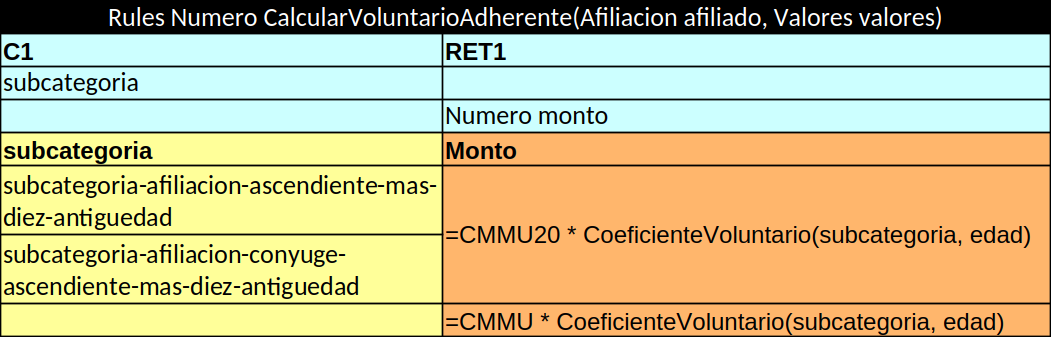
\includegraphics[width=1\textwidth]{voluntario.png}
    \caption{Cálculo de cuota de voluntario adherente}
    \label{tbl:cambio:original}
\end{table*}


% \begin{table*}[h]
%     \centering
%     \begin{tabular}{|p{7cm}|p{7cm}|}
%         \hline
%         \multicolumn{2}{|c|}{Rules Numero CalcularVoluntarioAdherente(Afiliacion afiliado, Valores valores)}                    \\ \hline
%         C1                                                              & RET1                                                \\ \hline
%         subcategoria                                                    &                                                     \\ \hline
%                                                                         & Numero monto                                        \\ \hline
%         subcategoria                                                    & Monto                                               \\ \hline
%         subcategoria-afiliacion-ascendiente-mas-diez-antiguedad         & =CMMU20 * CoeficienteVoluntario(subcategoria, edad) \\ \hline
%         subcategoria-afiliacion-conyuge-ascendiente-mas-diez-antiguedad &                                                     \\ \hline
%                                                                         & =CMMU * CoeficienteVoluntario(subcategoria, edad)   \\ \hline
%     \end{tabular}
%     \caption{Data from calcva.xls}
%     \label{tab:calcva}
% \end{table*}

% \begin{minted}{BNF}
% Rules <signatura>
% <signatura>::=<tipo> <nombre_tbl>(<pars>)
% <pars>::=<tipo> <nombre>
% \end{minted}


La fila 1 contiene el encabezado de la tabla.
En nuestro ejemplo: \tblcode{Rules} indica que la tabla contiene reglas,
\tblcode{Numero} es el tipo de retorno y \tblcode{CalcularVoluntarioAdherente(Afiliacion afiliado, Valores valores)} es el nombre de la tabla con sus dos parámetros.

La fila 2 define si la columna es una condición o valor de retorno, indicándose como  \tblcode{Cn} para la n-esima condición y \tblcode{RETn} para el n-esimo posible valor de retorno.
En el ejemplo, se indica que las columnas 1 y 2 corresponden a condiciones, y que en la 3 está el valor de retorno.

La fila 3 especifica la condición para cada columna en formato BEX \cite{openl-bex}.
Para \tblcode{C1} del ejemplo, se especifica \tblcode{subcategoria==valor}.
El lado izquierdo es inferido por nombre de uno de los atributos del parámetro \tblcode{afiliado} y el derecho se define en la fila 4.
La celda vacía para \tblcode{RET1} indica que no hay condiciones para ese retorno y se evalúa a \tblcode{Verdadero}.

% \begin{description}

    % \item[Fila 1: ] Contiene el encabezado de la tabla.
    %       En nuestro ejemplo: \tblcode{Rules} indica que la tabla contiene reglas,
    %       \tblcode{Numero} es el tipo de retorno y \tblcode{CalcularVoluntarioAdherente(Afiliacion afiliado, Valores valores)} es el nombre de la tabla con sus dos parámetros.

    % \item[Fila 2: ] Define si la/s columna/s es/son una condición o valor de retorno, indicándose como  \tblcode{Cn} para la n-esima condición y \tblcode{RET1} para el primer valor de retorno, respectivamente.
    %       En el ejemplo, se indica que las columnas 1 y 2 corresponden a condiciones, y que en la 3 está el valor de retorno.

    % \item[Fila 3: ] Especifica las condiciones para cada columna en formato BEX \cite{openl-bex}.
    %       Para \tblcode{C1} del ejemplo, se especifica \tblcode{subcategoria==valor}, donde el lado izquierdo es inferido por nombre de uno de los atributos del parámetro \tblcode{afiliado} y el derecho se define en la fila 4.
    %       La celda vacía para \tblcode{RET1} indica que no hay condiciones para ese retorno y se evalúa a \tblcode{Verdadero}.

    % \item[Fila 4: ] Define un parámetro por columna cuyos valores se definen a partir de la fila 6.
    %       Para \tblcode{C1} define de nombre \tblcode{valor} y tipo \tblcode{String}, y para \tblcode{RET1} el nombre \tblcode{monto} de tipo \tblcode{Numero}.

    % \item[Fila 5: ] Contiene nombres descriptivos para los parámetros, ignorados por el motor.

    % \item[Fila 6+:] Especifica los valores concretos para los parámetros.
    %       También pueden contener expresiones matemáticas o llamadas a otras reglas.

% \end{description}

La fila 4 define un parámetro por columna cuyos valores se definen a partir de la fila 6.
Para \tblcode{C1} define de nombre \tblcode{valor} y tipo \tblcode{String}, y para \tblcode{RET1} el nombre \tblcode{monto} de tipo \tblcode{Numero}.

La fila 5 contiene nombres descriptivos para los parámetros, ignorados por el motor.

Las filas 6, en adelante, especifican los valores concretos para los parámetros.
También pueden contener expresiones matemáticas o llamadas a otras reglas.
%
Para \tblcode{C1}, las filas 6 y 7 indican dos valores, que corresponden a ascendientes de primer grado con más de diez años de antigüedad y su cónyuge, respectivamente.
En ambos casos, el valor de \tblcode{RET1} es el mismo.
Se calcula como la multiplicación de un coeficiente, obtenido a partir de la tabla \tblcode{CoeficienteVoluntario} (no incluida en esta publicación), según la subcategoría y edad del afiliado, por el \acrshort{cmmu20}.
%
La fila 8 de \tblcode{C1} se encuentra vacía.
El motor interpreta que esta fila debe utilizarse por defecto para cualquier otro valor que no haya unificado aún.
El valor de retorno varía en este caso, ya que se utiliza el \acrshort{cmmu} en la multiplicación.

\subsection{Cuota de voluntario jubilado}

El cálculo del monto a abonar por jubilados es uno de los más complejos (junto con el caso de los voluntarios adherentes).
El mismo ocupa más de 150 líneas de código Java en la implementación original del \acrshort{si}.

Es cálculo inicia con el \cref{tbl:calculo:jubilado:1}.
Se debe notar un atajo utilizado en la notación para las expresiones de las dos condiciones, \tblcode{C1} y \tblcode{C2}.
Se coloca unicamente, el nombre del campo, que se obtiene del parámetro \tblcode{Afiliado}, cuando la expresión buscada es una igualdad con los valores que se colocaran en las celdas debajo.
Entonces, si el afiliado no tiene haber percibido actualizado, se retorna el valor calculado en el \cref{tbl:calculo:jubilado:sinhaber}. 
En caso de si tenerlo, 
el cálculo continua con el \cref{tbl:calculo:jubilado:sinconyuge} o con el \cref{tbl:calculo:jubilado:conconyuge}, dependiendo de si el afiliado tiene un cónyuge o conviviente que también sea titular en la obra social, o no.

\begin{table*}
    \centering
    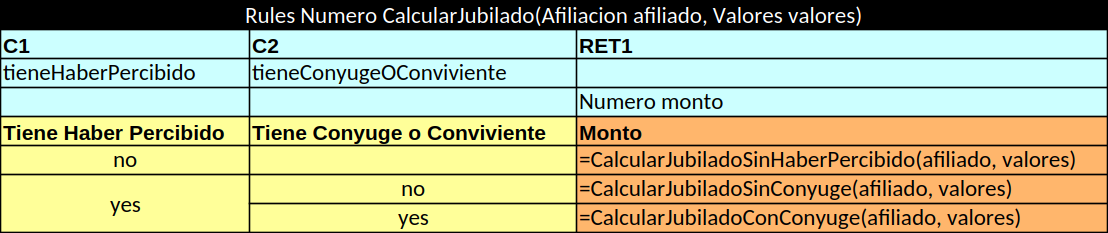
\includegraphics[width=.93\textwidth]{jubilado.png}
    \caption{Cálculo de cuota de jubilado}
    \label{tbl:calculo:jubilado:1}
\end{table*}

El cálculo del monto para un afiliado sin haber actualizado se muestra en el \cref{tbl:calculo:jubilado:sinhaber}.
Se toma como monto la cuota máxima de jubilado por un modificador, el cual se define dependiendo de si tiene un cónyuge o conviviente como afiliado familiar.
El caso para voluntario jubilado sin cónyuge titular (responsable de pago) es similar.
El mismo se trata en el \cref{tbl:calculo:jubilado:sinconyuge}.
La diferencia es que que se usa la fórmula de cálculo en base a su haber percibido \cref{tbl:calculo:jubilado:base}, en lugar de la cuota máxima de jubilado.

\begin{table*}
    \centering
    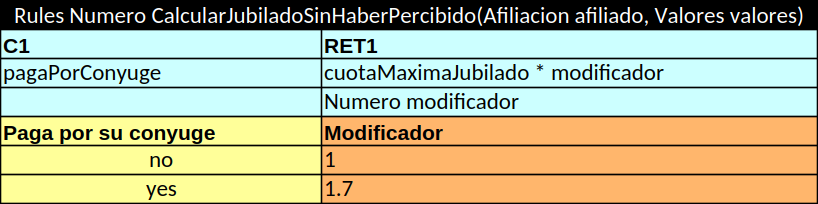
\includegraphics[width=0.70\textwidth]{jubiladoSinHaber.png}
    \caption{Cálculo de cuota de jubilado sin haber actualizado}
    \label{tbl:calculo:jubilado:sinhaber}
\end{table*}


\begin{table*}
    \centering
    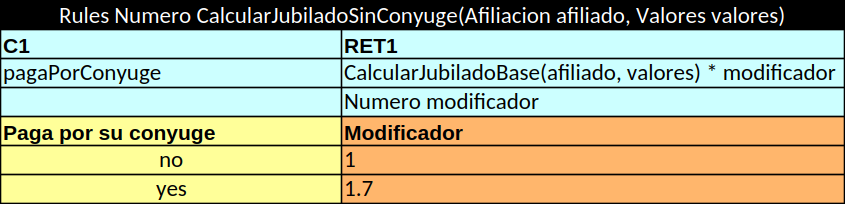
\includegraphics[width=0.71\textwidth]{jubiladoSinConyuge.png}
    \caption{Cálculo de cuota de jubilado sin cónyuge titular}
    \label{tbl:calculo:jubilado:sinconyuge}
\end{table*}

\begin{table*}
    \centering
    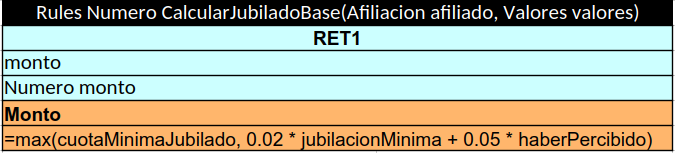
\includegraphics[width=0.63\textwidth]{base.png}
    \caption{Cálculo cuota base jubilado}
    \label{tbl:calculo:jubilado:base}
\end{table*}

El caso de voluntario jubilado con cónyuge titular requiere dos tablas. 
La primera se puede ver en el \cref{tbl:calculo:jubilado:conconyuge}.
En ella se comprueba si su cónyuge es también voluntario jubilado titular.
En caso de serlo, dependiendo de su condición, que debe estar habilitado o en su defecto moroso, y si es responsable de pago y tiene su haber percibido actualizado, se utiliza el \cref{tbl:calculo:jubilado:conyuge:responsable}.
Cabe aclarar que puede ser titular, pero no ser responsable de pago, si su cónyuge pague su cuota. 
En el \cref{tbl:calculo:jubilado:conyuge:responsable} se controla si el voluntario al que se le está cobrando, que tiene cónyuge que también es voluntario jubilado, es el de menor ingresos, para hacer el descuento en el monto.
El tratamiento de este caso puede parecer controlar de manera redundante algunas condiciones. 
Esto es por que el tratamiento de cada afiliado titular de hace de manera independiente, no como grupo familiar.

\begin{table*}
    \centering
    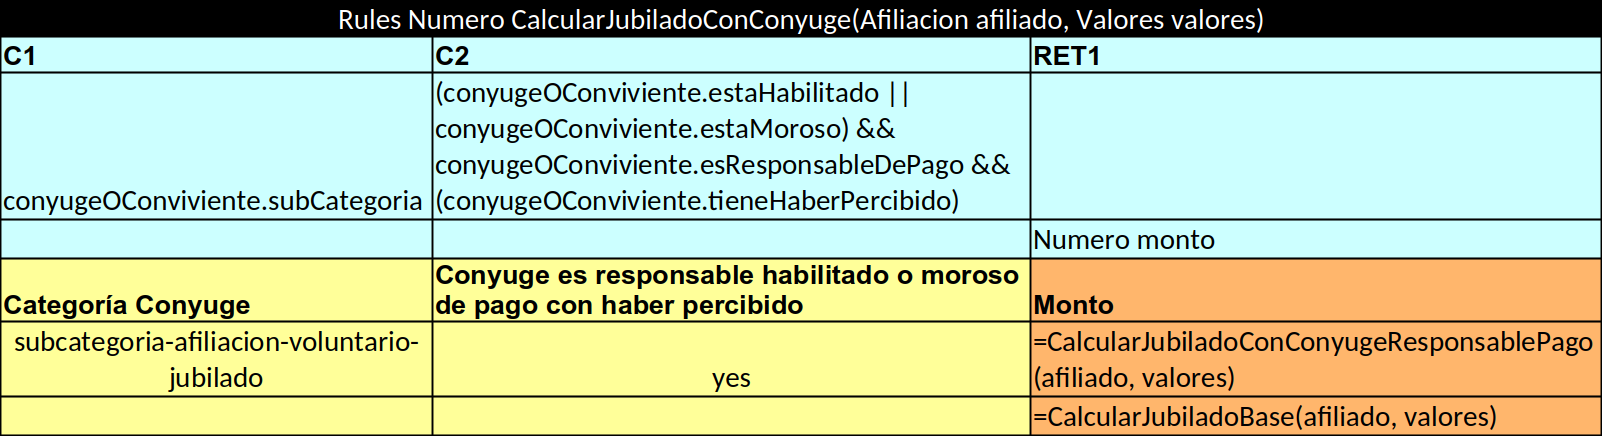
\includegraphics[width=1\textwidth]{jubiladoConConyuge.png}
    \caption{Cálculo de cuota de jubilado con cónyuge}
    \label{tbl:calculo:jubilado:conconyuge}
\end{table*}

\begin{table*}
    \centering
    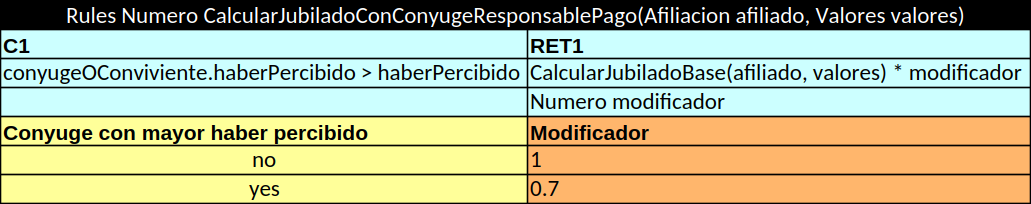
\includegraphics[width=0.85\textwidth]{jubiladoConConyugeResponsable.png}
    \caption{Cálculo cuota jubilado con cónyuge}
    \label{tbl:calculo:jubilado:conyuge:responsable}
\end{table*}

\subsection{Simulando un cambio}
\label{ssec:integracion:cambio}

Para ilustrar las ventajas de integrar el motor de reglas, consideremos la aplicación del siguiente cambio.

\emph{
El cálculo de la cuota de un afiliado agente \acrshort{unsl} con licencia será equivalente al 9\% del sueldo bruto que percibiría si estuviera en actividad. 
De igual forma, dicho monto no puede ser inferior a los porcentajes de la \acrshort{cmmu} que se utilizan en el cálculo anteriormente presentado para la subcategoría.
}

Para implementar el cambio, basta modificar la especificación en el \cref{tbl:cambio:original} para que quede como el \cref{tbl:cambio:cambiado}. 
En este último hay una fila adicional considerando el caso especial introducido para el afiliado agente \acrshort{unsl} con licencia.

\begin{table*}
    \centering
    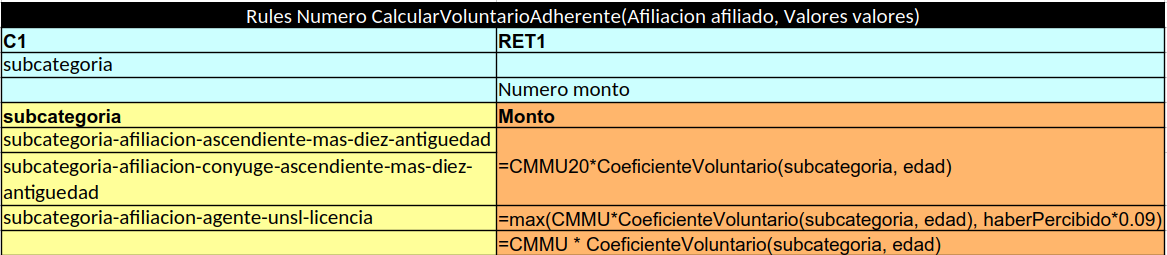
\includegraphics[width=1\textwidth]{voluntario_cambios.png}
    \caption{Cálculo modificado voluntario adherente modificado}
    \label{tbl:cambio:cambiado}
\end{table*}


\section{Resultados}
\label{sec:resultados}

Los resultados principales son mejoras en la mantenibilidad: en el esfuerzo requerido para materializar un cambio, y en la legibilidad del código fuente.

Para evaluar el esfuerzo requerido para implementar un cambio, consideremos dos escenarios para el cambio descrito en el \cref{ssec:integracion:cambio}: 
sobre el sistema original, o sobre el sistema con el motor de reglas integrado. 
En el primer escenario, el cambio implica la modificación/adición de unas 32 líneas de código.
Seguidamente, se debe volver a compilar y desplegar el sistema para que estos cambios sean efectivos.
%
En el segundo escenario, el cambio se materializa en el acto.
En tiempo de ejecución, el cambio es detectado y se generan nuevas clases wrapper, sin necesidad de volver a compilar el código fuente, o desplegar una nueva versión del sistema.


La legibilidad del código fuente se estudió utilizando como métrica cuantitativa la cantidad de líneas de código que corresponden a la totalidad de las líneas responsables del cálculo de las cuotas.
%
Para reducir el sesgo de formateo, se midieron las líneas de código utilizando dos formateadores distintos:
\begin{itemize}
    \item \href{https://github.com/google/google-java-format}{google-java-format} (GJF): un formateador que sigue la \href{https://google.github.io/styleguide/javaguide.html}{Guía de estilo de Java de Google}.
    \item Formateador de JDT LS, que es la implementación de \acrshort{lsp} de Java utilizada por la IDE de Eclipse.
\end{itemize}
Se consideraron dos versiones: la original, y la resultante luego de mejorar el original aplicando patrones de programación funcional (ver \cref{sec:metodologia}).
En el \cref{tbl:results} se pueden ver las líneas de código de ambas.
Se puede ver que más allá del formateador utilizado, la segunda posee un menor número de líneas.
%
Por otra parte, utilizando el motor de reglas se utilizan 143 filas en todas las tablas utilizadas para los cálculos. Esto es considerablemente menos que la mejor medición de líneas de código: 444.
%
\begin{table}[h]
    \centering
    \begin{tabular}{|c|c|c|}
        \hline
                  & GJF & JDT LS \\ \hline
        Original  & 573 & 556    \\ \hline
        Funcional & 512 & 444    \\ \hline
    \end{tabular}
    \caption{Cantidad de líneas de código}
    \label{tbl:results}
\end{table}



Conclusión y Trabajos Futuros (Times New Roman, 12, negrita) 
Esta sección debe explicitar las limitaciones del trabajo presentado y establecer una discusión sobre los resultados o conclusiones presentadas. Se debe realizar un análisis de los aportes del trabajo frente a otros anteriores si los hubiera. Además, se deben establecer cuestiones abiertas y probables líneas adicionales en el marco de los resultados obtenidos. Los trabajos futuros se deben relacionar con la superación de las limitaciones del trabajo presentado. Muchas veces es, junto con el título, la parte más leída y por lo tanto debe ser de fácil comprensión. (Times New Roman, 12).


\ifblind
    \begin{thanks}
Oculto para revisión.
\end{thanks}

\else
    \begin{thanks}
Agradecimientos (Times New Roman, 10, negrita) 
Si existiera, mencionarlos en forma concisa. Será escrito en fuente (Times New Roman, 10).
\end{thanks}

\fi

\printbibliography

\ifblind
    \begin{contact}
Oculto para revisión
\end{contact}

\else
    Datos de Contacto: (Times New Roman, 10, negrita) 
Nombre y Apellido. Institución. Dirección postal. E-mail. Serán escritos en fuente (Times New Roman, 10, Cursiva)

\fi
\end{document}
